\documentclass[1p]{elsarticle_modified}
%\bibliographystyle{elsarticle-num}

%\usepackage[colorlinks]{hyperref}
%\usepackage{abbrmath_seonhwa} %\Abb, \Ascr, \Acal ,\Abf, \Afrak
\usepackage{amsfonts}
\usepackage{amssymb}
\usepackage{amsmath}
\usepackage{amsthm}
\usepackage{scalefnt}
\usepackage{amsbsy}
\usepackage{kotex}
\usepackage{caption}
\usepackage{subfig}
\usepackage{color}
\usepackage{graphicx}
\usepackage{xcolor} %% white, black, red, green, blue, cyan, magenta, yellow
\usepackage{float}
\usepackage{setspace}
\usepackage{hyperref}

\usepackage{tikz}
\usetikzlibrary{arrows}

\usepackage{multirow}
\usepackage{array} % fixed length table
\usepackage{hhline}

%%%%%%%%%%%%%%%%%%%%%
\makeatletter
\renewcommand*\env@matrix[1][\arraystretch]{%
	\edef\arraystretch{#1}%
	\hskip -\arraycolsep
	\let\@ifnextchar\new@ifnextchar
	\array{*\c@MaxMatrixCols c}}
\makeatother %https://tex.stackexchange.com/questions/14071/how-can-i-increase-the-line-spacing-in-a-matrix
%%%%%%%%%%%%%%%

\usepackage[normalem]{ulem}

\newcommand{\msout}[1]{\ifmmode\text{\sout{\ensuremath{#1}}}\else\sout{#1}\fi}
%SOURCE: \msout is \stkout macro in https://tex.stackexchange.com/questions/20609/strikeout-in-math-mode

\newcommand{\cancel}[1]{
	\ifmmode
	{\color{red}\msout{#1}}
	\else
	{\color{red}\sout{#1}}
	\fi
}

\newcommand{\add}[1]{
	{\color{blue}\uwave{#1}}
}

\newcommand{\replace}[2]{
	\ifmmode
	{\color{red}\msout{#1}}{\color{blue}\uwave{#2}}
	\else
	{\color{red}\sout{#1}}{\color{blue}\uwave{#2}}
	\fi
}

\newcommand{\Sol}{\mathcal{S}} %segment
\newcommand{\D}{D} %diagram
\newcommand{\A}{\mathcal{A}} %arc


%%%%%%%%%%%%%%%%%%%%%%%%%%%%%5 test

\def\sl{\operatorname{\textup{SL}}(2,\Cbb)}
\def\psl{\operatorname{\textup{PSL}}(2,\Cbb)}
\def\quan{\mkern 1mu \triangleright \mkern 1mu}

\theoremstyle{definition}
\newtheorem{thm}{Theorem}[section]
\newtheorem{prop}[thm]{Proposition}
\newtheorem{lem}[thm]{Lemma}
\newtheorem{ques}[thm]{Question}
\newtheorem{cor}[thm]{Corollary}
\newtheorem{defn}[thm]{Definition}
\newtheorem{exam}[thm]{Example}
\newtheorem{rmk}[thm]{Remark}
\newtheorem{alg}[thm]{Algorithm}

\newcommand{\I}{\sqrt{-1}}
\begin{document}

%\begin{frontmatter}
%
%\title{Boundary parabolic representations of knots up to 8 crossings}
%
%%% Group authors per affiliation:
%\author{Yunhi Cho} 
%\address{Department of Mathematics, University of Seoul, Seoul, Korea}
%\ead{yhcho@uos.ac.kr}
%
%
%\author{Seonhwa Kim} %\fnref{s_kim}}
%\address{Center for Geometry and Physics, Institute for Basic Science, Pohang, 37673, Korea}
%\ead{ryeona17@ibs.re.kr}
%
%\author{Hyuk Kim}
%\address{Department of Mathematical Sciences, Seoul National University, Seoul 08826, Korea}
%\ead{hyukkim@snu.ac.kr}
%
%\author{Seokbeom Yoon}
%\address{Department of Mathematical Sciences, Seoul National University, Seoul, 08826,  Korea}
%\ead{sbyoon15@snu.ac.kr}
%
%\begin{abstract}
%We find all boundary parabolic representation of knots up to 8 crossings.
%
%\end{abstract}
%\begin{keyword}
%    \MSC[2010] 57M25 
%\end{keyword}
%
%\end{frontmatter}

%\linenumbers
%\tableofcontents
%
\newcommand\colored[1]{\textcolor{white}{\rule[-0.35ex]{0.8em}{1.4ex}}\kern-0.8em\color{red} #1}%
%\newcommand\colored[1]{\textcolor{white}{ #1}\kern-2.17ex	\textcolor{white}{ #1}\kern-1.81ex	\textcolor{white}{ #1}\kern-2.15ex\color{red}#1	}

{\Large $\underline{12n_{0678}~(K12n_{0678})}$}

\setlength{\tabcolsep}{10pt}
\renewcommand{\arraystretch}{1.6}
\vspace{1cm}\begin{tabular}{m{100pt}>{\centering\arraybackslash}m{274pt}}
\multirow{5}{120pt}{
	\centering
	\includegraphics[width=112pt]{../../../GIT/diagram.site/Diagrams/png/2767_12n_0678.png}\\
\ \ \ A knot diagram\footnotemark}&
\allowdisplaybreaks
\textbf{Linearized knot diagam} \\
\cline{2-2}
 &
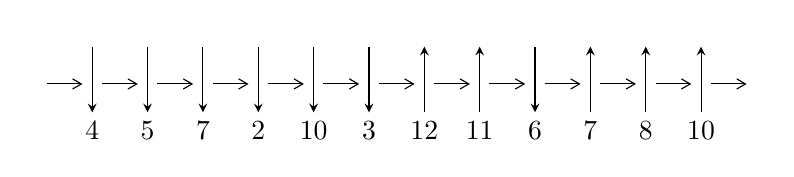
\begin{tikzpicture}[x=20pt, y=17pt]
	% nodes
	\node (C0) at (0, 0) {};
	\node (C1) at (1, 0) {};
	\node (C1U) at (1, +1) {};
	\node (C1D) at (1, -1) {4};

	\node (C2) at (2, 0) {};
	\node (C2U) at (2, +1) {};
	\node (C2D) at (2, -1) {5};

	\node (C3) at (3, 0) {};
	\node (C3U) at (3, +1) {};
	\node (C3D) at (3, -1) {7};

	\node (C4) at (4, 0) {};
	\node (C4U) at (4, +1) {};
	\node (C4D) at (4, -1) {2};

	\node (C5) at (5, 0) {};
	\node (C5U) at (5, +1) {};
	\node (C5D) at (5, -1) {10};

	\node (C6) at (6, 0) {};
	\node (C6U) at (6, +1) {};
	\node (C6D) at (6, -1) {3};

	\node (C7) at (7, 0) {};
	\node (C7U) at (7, +1) {};
	\node (C7D) at (7, -1) {12};

	\node (C8) at (8, 0) {};
	\node (C8U) at (8, +1) {};
	\node (C8D) at (8, -1) {11};

	\node (C9) at (9, 0) {};
	\node (C9U) at (9, +1) {};
	\node (C9D) at (9, -1) {6};

	\node (C10) at (10, 0) {};
	\node (C10U) at (10, +1) {};
	\node (C10D) at (10, -1) {7};

	\node (C11) at (11, 0) {};
	\node (C11U) at (11, +1) {};
	\node (C11D) at (11, -1) {8};

	\node (C12) at (12, 0) {};
	\node (C12U) at (12, +1) {};
	\node (C12D) at (12, -1) {10};
	\node (C13) at (13, 0) {};

	% arrows
	\draw[->,>={angle 60}]
	(C0) edge (C1) (C1) edge (C2) (C2) edge (C3) (C3) edge (C4) (C4) edge (C5) (C5) edge (C6) (C6) edge (C7) (C7) edge (C8) (C8) edge (C9) (C9) edge (C10) (C10) edge (C11) (C11) edge (C12) (C12) edge (C13) ;	\draw[->,>=stealth]
	(C1U) edge (C1D) (C2U) edge (C2D) (C3U) edge (C3D) (C4U) edge (C4D) (C5U) edge (C5D) (C6U) edge (C6D) (C7D) edge (C7U) (C8D) edge (C8U) (C9U) edge (C9D) (C10D) edge (C10U) (C11D) edge (C11U) (C12D) edge (C12U) ;
	\end{tikzpicture} \\
\hhline{~~} \\& 
\textbf{Solving Sequence} \\ \cline{2-2} 
 &
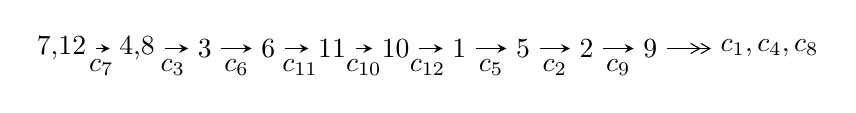
\begin{tikzpicture}[x=23pt, y=7pt]
	% node
	\node (A0) at (-1/8, 0) {7,12};
	\node (A1) at (17/16, 0) {4,8};
	\node (A2) at (17/8, 0) {3};
	\node (A3) at (25/8, 0) {6};
	\node (A4) at (33/8, 0) {11};
	\node (A5) at (41/8, 0) {10};
	\node (A6) at (49/8, 0) {1};
	\node (A7) at (57/8, 0) {5};
	\node (A8) at (65/8, 0) {2};
	\node (A9) at (73/8, 0) {9};
	\node (C1) at (1/2, -1) {$c_{7}$};
	\node (C2) at (13/8, -1) {$c_{3}$};
	\node (C3) at (21/8, -1) {$c_{6}$};
	\node (C4) at (29/8, -1) {$c_{11}$};
	\node (C5) at (37/8, -1) {$c_{10}$};
	\node (C6) at (45/8, -1) {$c_{12}$};
	\node (C7) at (53/8, -1) {$c_{5}$};
	\node (C8) at (61/8, -1) {$c_{2}$};
	\node (C9) at (69/8, -1) {$c_{9}$};
	\node (A10) at (11, 0) {$c_{1},c_{4},c_{8}$};

	% edge
	\draw[->,>=stealth]	
	(A0) edge (A1) (A1) edge (A2) (A2) edge (A3) (A3) edge (A4) (A4) edge (A5) (A5) edge (A6) (A6) edge (A7) (A7) edge (A8) (A8) edge (A9) ;
	\draw[->>,>={angle 60}]	
	(A9) edge (A10);
\end{tikzpicture} \\ 

\end{tabular} \\

\footnotetext{
The image of knot diagram is generated by the software ``\textbf{Draw programme}" developed by Andrew Bartholomew(\url{http://www.layer8.co.uk/maths/draw/index.htm\#Running-draw}), where we modified some parts for our purpose(\url{https://github.com/CATsTAILs/LinksPainter}).
}\phantom \\ \newline 
\centering \textbf{Ideals for irreducible components\footnotemark of $X_{\text{par}}$} 
 
\begin{align*}
I^u_{1}&=\langle 
-171832171743933 u^{44}+565195223234702 u^{43}+\cdots+319912709247818 b-45090425568559,\\
\phantom{I^u_{1}}&\phantom{= \langle  }221527977237717 u^{44}-489493690784658 u^{43}+\cdots+319912709247818 a+1085130159951208,\\
\phantom{I^u_{1}}&\phantom{= \langle  }u^{45}-3 u^{44}+\cdots-8 u+1\rangle \\
I^u_{2}&=\langle 
- a u+b- u,\;u^2 a+a^2+a u- u^2+4 a,\;u^3+u^2+2 u+1\rangle \\
\\
\end{align*}
\raggedright * 2 irreducible components of $\dim_{\mathbb{C}}=0$, with total 51 representations.\\
\footnotetext{All coefficients of polynomials are rational numbers. But the coefficients are sometimes approximated in decimal forms when there is not enough margin.}
\newpage
\renewcommand{\arraystretch}{1}
\centering \section*{I. $I^u_{1}= \langle -1.72\times10^{14} u^{44}+5.65\times10^{14} u^{43}+\cdots+3.20\times10^{14} b-4.51\times10^{13},\;2.22\times10^{14} u^{44}-4.89\times10^{14} u^{43}+\cdots+3.20\times10^{14} a+1.09\times10^{15},\;u^{45}-3 u^{44}+\cdots-8 u+1 \rangle$}
\flushleft \textbf{(i) Arc colorings}\\
\begin{tabular}{m{7pt} m{180pt} m{7pt} m{180pt} }
\flushright $a_{7}=$&$\begin{pmatrix}1\\0\end{pmatrix}$ \\
\flushright $a_{12}=$&$\begin{pmatrix}0\\u\end{pmatrix}$ \\
\flushright $a_{4}=$&$\begin{pmatrix}-0.692464 u^{44}+1.53009 u^{43}+\cdots-21.6689 u-3.39196\\0.537122 u^{44}-1.76672 u^{43}+\cdots+4.08754 u+0.140946\end{pmatrix}$ \\
\flushright $a_{8}=$&$\begin{pmatrix}1\\- u^2\end{pmatrix}$ \\
\flushright $a_{3}=$&$\begin{pmatrix}-0.155342 u^{44}-0.236632 u^{43}+\cdots-17.5814 u-3.25101\\0.537122 u^{44}-1.76672 u^{43}+\cdots+4.08754 u+0.140946\end{pmatrix}$ \\
\flushright $a_{6}=$&$\begin{pmatrix}1.72119 u^{44}-3.14555 u^{43}+\cdots+18.4989 u+1.81534\\-2.01801 u^{44}+5.92336 u^{43}+\cdots-15.5848 u+1.72119\end{pmatrix}$ \\
\flushright $a_{11}=$&$\begin{pmatrix}- u\\u^3+u\end{pmatrix}$ \\
\flushright $a_{10}=$&$\begin{pmatrix}- u^3-2 u\\u^3+u\end{pmatrix}$ \\
\flushright $a_{1}=$&$\begin{pmatrix}u^7+4 u^5+4 u^3\\- u^7-3 u^5-2 u^3+u\end{pmatrix}$ \\
\flushright $a_{5}=$&$\begin{pmatrix}-0.470191 u^{44}+1.87005 u^{43}+\cdots+7.18359 u+3.39261\\-0.462878 u^{44}+1.23328 u^{43}+\cdots-3.91246 u+0.140946\end{pmatrix}$ \\
\flushright $a_{2}=$&$\begin{pmatrix}-1.21496 u^{44}+3.02326 u^{43}+\cdots-22.9486 u-0.0362322\\0.462878 u^{44}-1.23328 u^{43}+\cdots+3.91246 u-0.140946\end{pmatrix}$ \\
\flushright $a_{9}=$&$\begin{pmatrix}u^2+1\\- u^4-2 u^2\end{pmatrix}$\\&\end{tabular}
\flushleft \textbf{(ii) Obstruction class $= -1$}\\~\\
\flushleft \textbf{(iii) Cusp Shapes $= -\frac{124420232195109}{159956354623909} u^{44}+\frac{585183168556345}{319912709247818} u^{43}+\cdots-\frac{6164660264148967}{319912709247818} u-\frac{3111644555281919}{319912709247818}$}\\~\\
\newpage\renewcommand{\arraystretch}{1}
\flushleft \textbf{(iv) u-Polynomials at the component}\newline \\
\begin{tabular}{m{50pt}|m{274pt}}
Crossings & \hspace{64pt}u-Polynomials at each crossing \\
\hline $$\begin{aligned}c_{1},c_{2},c_{4}\end{aligned}$$&$\begin{aligned}
&u^{45}-4 u^{44}+\cdots+3 u-1
\end{aligned}$\\
\hline $$\begin{aligned}c_{3},c_{6}\end{aligned}$$&$\begin{aligned}
&u^{45}+4 u^{44}+\cdots- u+1
\end{aligned}$\\
\hline $$\begin{aligned}c_{5},c_{9}\end{aligned}$$&$\begin{aligned}
&u^{45}+3 u^{44}+\cdots+160 u+64
\end{aligned}$\\
\hline $$\begin{aligned}c_{7},c_{8},c_{11}\end{aligned}$$&$\begin{aligned}
&u^{45}+3 u^{44}+\cdots-8 u-1
\end{aligned}$\\
\hline $$\begin{aligned}c_{10}\end{aligned}$$&$\begin{aligned}
&u^{45}-3 u^{44}+\cdots-542 u-97
\end{aligned}$\\
\hline $$\begin{aligned}c_{12}\end{aligned}$$&$\begin{aligned}
&u^{45}+19 u^{44}+\cdots+653792 u-13633
\end{aligned}$\\
\hline
\end{tabular}\\~\\
\newpage\renewcommand{\arraystretch}{1}
\flushleft \textbf{(v) Riley Polynomials at the component}\newline \\
\begin{tabular}{m{50pt}|m{274pt}}
Crossings & \hspace{64pt}Riley Polynomials at each crossing \\
\hline $$\begin{aligned}c_{1},c_{2},c_{4}\end{aligned}$$&$\begin{aligned}
&y^{45}-34 y^{44}+\cdots+5 y-1
\end{aligned}$\\
\hline $$\begin{aligned}c_{3},c_{6}\end{aligned}$$&$\begin{aligned}
&y^{45}-6 y^{44}+\cdots+5 y-1
\end{aligned}$\\
\hline $$\begin{aligned}c_{5},c_{9}\end{aligned}$$&$\begin{aligned}
&y^{45}+35 y^{44}+\cdots+58368 y-4096
\end{aligned}$\\
\hline $$\begin{aligned}c_{7},c_{8},c_{11}\end{aligned}$$&$\begin{aligned}
&y^{45}+37 y^{44}+\cdots+120 y-1
\end{aligned}$\\
\hline $$\begin{aligned}c_{10}\end{aligned}$$&$\begin{aligned}
&y^{45}-39 y^{44}+\cdots+1081792 y-9409
\end{aligned}$\\
\hline $$\begin{aligned}c_{12}\end{aligned}$$&$\begin{aligned}
&y^{45}-59 y^{44}+\cdots+530299074808 y-185858689
\end{aligned}$\\
\hline
\end{tabular}\\~\\
\newpage\flushleft \textbf{(vi) Complex Volumes and Cusp Shapes}
$$\begin{array}{c|c|c}  
\text{Solutions to }I^u_{1}& \I (\text{vol} + \sqrt{-1}CS) & \text{Cusp shape}\\
 \hline 
\begin{aligned}
u &= -0.583612 + 0.749370 I \\
a &= -0.145378 - 1.180080 I \\
b &= \phantom{-}0.314212 + 0.693704 I\end{aligned}
 & -0.22746 - 3.52607 I & -0.53223 + 9.05892 I \\ \hline\begin{aligned}
u &= -0.583612 - 0.749370 I \\
a &= -0.145378 + 1.180080 I \\
b &= \phantom{-}0.314212 - 0.693704 I\end{aligned}
 & -0.22746 + 3.52607 I & -0.53223 - 9.05892 I \\ \hline\begin{aligned}
u &= \phantom{-}0.884188 + 0.167276 I \\
a &= -1.44217 + 3.00622 I \\
b &= \phantom{-}1.01437 - 1.10209 I\end{aligned}
 & \phantom{-}4.46171 + 9.77082 I & -1.55814 - 6.22355 I \\ \hline\begin{aligned}
u &= \phantom{-}0.884188 - 0.167276 I \\
a &= -1.44217 - 3.00622 I \\
b &= \phantom{-}1.01437 + 1.10209 I\end{aligned}
 & \phantom{-}4.46171 - 9.77082 I & -1.55814 + 6.22355 I \\ \hline\begin{aligned}
u &= -0.862556 + 0.189586 I \\
a &= -0.10994 + 1.47934 I \\
b &= -0.099189 - 0.621407 I\end{aligned}
 & \phantom{-}1.49082 - 1.15898 I & \phantom{-}5.48142 + 4.79165 I \\ \hline\begin{aligned}
u &= -0.862556 - 0.189586 I \\
a &= -0.10994 - 1.47934 I \\
b &= -0.099189 + 0.621407 I\end{aligned}
 & \phantom{-}1.49082 + 1.15898 I & \phantom{-}5.48142 - 4.79165 I \\ \hline\begin{aligned}
u &= \phantom{-}0.879134 + 0.073302 I \\
a &= \phantom{-}1.69262 - 2.92394 I \\
b &= -1.05605 + 1.10417 I\end{aligned}
 & \phantom{-}8.52509 + 4.00354 I & \phantom{-}1.85103 - 2.75584 I \\ \hline\begin{aligned}
u &= \phantom{-}0.879134 - 0.073302 I \\
a &= \phantom{-}1.69262 + 2.92394 I \\
b &= -1.05605 - 1.10417 I\end{aligned}
 & \phantom{-}8.52509 - 4.00354 I & \phantom{-}1.85103 + 2.75584 I \\ \hline\begin{aligned}
u &= \phantom{-}0.834305 + 0.026519 I \\
a &= -2.03456 - 2.80224 I \\
b &= \phantom{-}1.11558 + 1.09067 I\end{aligned}
 & \phantom{-}4.18745 + 1.80014 I & \phantom{-}0.034492 - 1.194140 I \\ \hline\begin{aligned}
u &= \phantom{-}0.834305 - 0.026519 I \\
a &= -2.03456 + 2.80224 I \\
b &= \phantom{-}1.11558 - 1.09067 I\end{aligned}
 & \phantom{-}4.18745 - 1.80014 I & \phantom{-}0.034492 + 1.194140 I\\
 \hline 
 \end{array}$$\newpage$$\begin{array}{c|c|c}  
\text{Solutions to }I^u_{1}& \I (\text{vol} + \sqrt{-1}CS) & \text{Cusp shape}\\
 \hline 
\begin{aligned}
u &= \phantom{-}0.481295 + 1.085350 I \\
a &= -1.52416 - 1.39190 I \\
b &= \phantom{-}0.840283 + 1.091050 I\end{aligned}
 & \phantom{-}1.64682 - 4.91710 I & -3.75732 + 2.86803 I \\ \hline\begin{aligned}
u &= \phantom{-}0.481295 - 1.085350 I \\
a &= -1.52416 + 1.39190 I \\
b &= \phantom{-}0.840283 - 1.091050 I\end{aligned}
 & \phantom{-}1.64682 + 4.91710 I & -3.75732 - 2.86803 I \\ \hline\begin{aligned}
u &= -0.027576 + 1.213260 I \\
a &= \phantom{-}0.097830 + 0.955725 I \\
b &= \phantom{-}0.987113 - 0.071189 I\end{aligned}
 & -4.06865 - 0.00938 I & -7.42868 + 0. I\phantom{ +0.000000I} \\ \hline\begin{aligned}
u &= -0.027576 - 1.213260 I \\
a &= \phantom{-}0.097830 - 0.955725 I \\
b &= \phantom{-}0.987113 + 0.071189 I\end{aligned}
 & -4.06865 + 0.00938 I & -7.42868 + 0. I\phantom{ +0.000000I} \\ \hline\begin{aligned}
u &= -0.310904 + 1.181390 I \\
a &= -0.21426 - 1.54867 I \\
b &= \phantom{-}0.294215 + 0.670186 I\end{aligned}
 & -1.38332 - 2.86199 I & \phantom{-0.000000 -}0. + 3.33644 I \\ \hline\begin{aligned}
u &= -0.310904 - 1.181390 I \\
a &= -0.21426 + 1.54867 I \\
b &= \phantom{-}0.294215 - 0.670186 I\end{aligned}
 & -1.38332 + 2.86199 I & \phantom{-0.000000 } 0. - 3.33644 I \\ \hline\begin{aligned}
u &= \phantom{-}0.159859 + 1.260150 I \\
a &= \phantom{-}1.07101 - 1.51572 I \\
b &= -1.63864 + 0.16074 I\end{aligned}
 & -11.89460 + 2.24035 I & -8.35575 + 0. I\phantom{ +0.000000I} \\ \hline\begin{aligned}
u &= \phantom{-}0.159859 - 1.260150 I \\
a &= \phantom{-}1.07101 + 1.51572 I \\
b &= -1.63864 - 0.16074 I\end{aligned}
 & -11.89460 - 2.24035 I & -8.35575 + 0. I\phantom{ +0.000000I} \\ \hline\begin{aligned}
u &= \phantom{-}0.433209 + 1.205320 I \\
a &= \phantom{-}1.56995 + 1.36216 I \\
b &= -0.89067 - 1.16692 I\end{aligned}
 & \phantom{-}5.04167 + 0.68814 I & \phantom{-0.000000 } 0 \\ \hline\begin{aligned}
u &= \phantom{-}0.433209 - 1.205320 I \\
a &= \phantom{-}1.56995 - 1.36216 I \\
b &= -0.89067 + 1.16692 I\end{aligned}
 & \phantom{-}5.04167 - 0.68814 I & \phantom{-0.000000 } 0\\
 \hline 
 \end{array}$$\newpage$$\begin{array}{c|c|c}  
\text{Solutions to }I^u_{1}& \I (\text{vol} + \sqrt{-1}CS) & \text{Cusp shape}\\
 \hline 
\begin{aligned}
u &= -0.091883 + 1.292420 I \\
a &= \phantom{-}0.68882 + 2.04860 I \\
b &= \phantom{-}0.100880 - 0.832088 I\end{aligned}
 & -5.73773 - 2.01190 I & \phantom{-0.000000 } 0 \\ \hline\begin{aligned}
u &= -0.091883 - 1.292420 I \\
a &= \phantom{-}0.68882 - 2.04860 I \\
b &= \phantom{-}0.100880 + 0.832088 I\end{aligned}
 & -5.73773 + 2.01190 I & \phantom{-0.000000 } 0 \\ \hline\begin{aligned}
u &= \phantom{-}0.378074 + 1.248800 I \\
a &= -0.30888 + 2.43252 I \\
b &= \phantom{-}1.23412 - 0.93095 I\end{aligned}
 & \phantom{-}0.40714 + 2.55603 I & \phantom{-0.000000 } 0 \\ \hline\begin{aligned}
u &= \phantom{-}0.378074 - 1.248800 I \\
a &= -0.30888 - 2.43252 I \\
b &= \phantom{-}1.23412 + 0.93095 I\end{aligned}
 & \phantom{-}0.40714 - 2.55603 I & \phantom{-0.000000 } 0 \\ \hline\begin{aligned}
u &= -0.233067 + 1.286920 I \\
a &= -1.54727 - 1.27295 I \\
b &= -0.472121 + 0.195549 I\end{aligned}
 & -4.28958 - 3.06247 I & -27.0240 + 0. I\phantom{ +0.000000I} \\ \hline\begin{aligned}
u &= -0.233067 - 1.286920 I \\
a &= -1.54727 + 1.27295 I \\
b &= -0.472121 - 0.195549 I\end{aligned}
 & -4.28958 + 3.06247 I & -27.0240 + 0. I\phantom{ +0.000000I} \\ \hline\begin{aligned}
u &= \phantom{-}0.376537 + 1.291220 I \\
a &= -1.67227 - 1.26273 I \\
b &= \phantom{-}0.99238 + 1.22341 I\end{aligned}
 & \phantom{-}0.08117 + 6.15166 I & \phantom{-0.000000 } 0 \\ \hline\begin{aligned}
u &= \phantom{-}0.376537 - 1.291220 I \\
a &= -1.67227 + 1.26273 I \\
b &= \phantom{-}0.99238 - 1.22341 I\end{aligned}
 & \phantom{-}0.08117 - 6.15166 I & \phantom{-0.000000 } 0 \\ \hline\begin{aligned}
u &= -0.594574 + 0.259179 I \\
a &= -0.442778 + 1.247600 I \\
b &= -0.223270 - 0.529291 I\end{aligned}
 & \phantom{-}1.36466 - 0.79548 I & \phantom{-}4.15835 + 2.62510 I \\ \hline\begin{aligned}
u &= -0.594574 - 0.259179 I \\
a &= -0.442778 - 1.247600 I \\
b &= -0.223270 + 0.529291 I\end{aligned}
 & \phantom{-}1.36466 + 0.79548 I & \phantom{-}4.15835 - 2.62510 I\\
 \hline 
 \end{array}$$\newpage$$\begin{array}{c|c|c}  
\text{Solutions to }I^u_{1}& \I (\text{vol} + \sqrt{-1}CS) & \text{Cusp shape}\\
 \hline 
\begin{aligned}
u &= -0.173829 + 1.352770 I \\
a &= -0.626070 + 0.431699 I \\
b &= -0.604107 - 0.273968 I\end{aligned}
 & -3.74207 - 3.36112 I & \phantom{-0.000000 } 0 \\ \hline\begin{aligned}
u &= -0.173829 - 1.352770 I \\
a &= -0.626070 - 0.431699 I \\
b &= -0.604107 + 0.273968 I\end{aligned}
 & -3.74207 + 3.36112 I & \phantom{-0.000000 } 0 \\ \hline\begin{aligned}
u &= -0.615344\phantom{ +0.000000I} \\
a &= -2.94504\phantom{ +0.000000I} \\
b &= -0.368354\phantom{ +0.000000I}\end{aligned}
 & -0.259777\phantom{ +0.000000I} & -41.6450\phantom{ +0.000000I} \\ \hline\begin{aligned}
u &= \phantom{-}0.399717 + 1.327110 I \\
a &= \phantom{-}0.22643 - 2.45843 I \\
b &= -1.17155 + 1.01534 I\end{aligned}
 & \phantom{-}4.14207 + 8.58803 I & \phantom{-0.000000 } 0 \\ \hline\begin{aligned}
u &= \phantom{-}0.399717 - 1.327110 I \\
a &= \phantom{-}0.22643 + 2.45843 I \\
b &= -1.17155 - 1.01534 I\end{aligned}
 & \phantom{-}4.14207 - 8.58803 I & \phantom{-0.000000 } 0 \\ \hline\begin{aligned}
u &= -0.40967 + 1.36131 I \\
a &= \phantom{-}0.064099 + 1.291930 I \\
b &= -0.432795 - 0.645865 I\end{aligned}
 & -3.33493 - 5.79576 I & \phantom{-0.000000 } 0 \\ \hline\begin{aligned}
u &= -0.40967 - 1.36131 I \\
a &= \phantom{-}0.064099 - 1.291930 I \\
b &= -0.432795 + 0.645865 I\end{aligned}
 & -3.33493 + 5.79576 I & \phantom{-0.000000 } 0 \\ \hline\begin{aligned}
u &= \phantom{-}0.38534 + 1.38238 I \\
a &= -0.15294 + 2.46124 I \\
b &= \phantom{-}1.12554 - 1.06328 I\end{aligned}
 & -0.4279 + 14.3330 I & \phantom{-0.000000 } 0 \\ \hline\begin{aligned}
u &= \phantom{-}0.38534 - 1.38238 I \\
a &= -0.15294 - 2.46124 I \\
b &= \phantom{-}1.12554 + 1.06328 I\end{aligned}
 & -0.4279 - 14.3330 I & \phantom{-0.000000 } 0 \\ \hline\begin{aligned}
u &= -0.11768 + 1.50035 I \\
a &= -0.220688 - 0.588458 I \\
b &= \phantom{-}0.779647 + 0.534509 I\end{aligned}
 & -7.68575 - 5.74695 I & \phantom{-0.000000 } 0\\
 \hline 
 \end{array}$$\newpage$$\begin{array}{c|c|c}  
\text{Solutions to }I^u_{1}& \I (\text{vol} + \sqrt{-1}CS) & \text{Cusp shape}\\
 \hline 
\begin{aligned}
u &= -0.11768 - 1.50035 I \\
a &= -0.220688 + 0.588458 I \\
b &= \phantom{-}0.779647 - 0.534509 I\end{aligned}
 & -7.68575 + 5.74695 I & \phantom{-0.000000 } 0 \\ \hline\begin{aligned}
u &= \phantom{-}0.466619\phantom{ +0.000000I} \\
a &= \phantom{-}4.22060\phantom{ +0.000000I} \\
b &= -1.54831\phantom{ +0.000000I}\end{aligned}
 & -8.02557\phantom{ +0.000000I} & -22.5480\phantom{ +0.000000I} \\ \hline\begin{aligned}
u &= -0.280147 + 0.187854 I \\
a &= \phantom{-}2.57065 + 1.29057 I \\
b &= \phantom{-}0.441345 - 0.382694 I\end{aligned}
 & -1.25055 - 0.68721 I & -6.23111 - 2.03128 I \\ \hline\begin{aligned}
u &= -0.280147 - 0.187854 I \\
a &= \phantom{-}2.57065 - 1.29057 I \\
b &= \phantom{-}0.441345 + 0.382694 I\end{aligned}
 & -1.25055 + 0.68721 I & -6.23111 + 2.03128 I \\ \hline\begin{aligned}
u &= \phantom{-}0.0963991\phantom{ +0.000000I} \\
a &= -5.35560\phantom{ +0.000000I} \\
b &= \phantom{-}0.614065\phantom{ +0.000000I}\end{aligned}
 & -0.870395\phantom{ +0.000000I} & -12.0080\phantom{ +0.000000I}\\
 \hline 
 \end{array}$$\newpage\newpage\renewcommand{\arraystretch}{1}
\centering \section*{II. $I^u_{2}= \langle - a u+b- u,\;u^2 a+a^2+a u- u^2+4 a,\;u^3+u^2+2 u+1 \rangle$}
\flushleft \textbf{(i) Arc colorings}\\
\begin{tabular}{m{7pt} m{180pt} m{7pt} m{180pt} }
\flushright $a_{7}=$&$\begin{pmatrix}1\\0\end{pmatrix}$ \\
\flushright $a_{12}=$&$\begin{pmatrix}0\\u\end{pmatrix}$ \\
\flushright $a_{4}=$&$\begin{pmatrix}a\\a u+u\end{pmatrix}$ \\
\flushright $a_{8}=$&$\begin{pmatrix}1\\- u^2\end{pmatrix}$ \\
\flushright $a_{3}=$&$\begin{pmatrix}a u+a+u\\a u+u\end{pmatrix}$ \\
\flushright $a_{6}=$&$\begin{pmatrix}u^2- a+u+1\\- a u- u-1\end{pmatrix}$ \\
\flushright $a_{11}=$&$\begin{pmatrix}- u\\- u^2- u-1\end{pmatrix}$ \\
\flushright $a_{10}=$&$\begin{pmatrix}u^2+1\\- u^2- u-1\end{pmatrix}$ \\
\flushright $a_{1}=$&$\begin{pmatrix}-1\\0\end{pmatrix}$ \\
\flushright $a_{5}=$&$\begin{pmatrix}u^2- a+u+1\\- a u- u-1\end{pmatrix}$ \\
\flushright $a_{2}=$&$\begin{pmatrix}a u+u^2- a+2 u\\- a u- u-1\end{pmatrix}$ \\
\flushright $a_{9}=$&$\begin{pmatrix}u^2+1\\- u^2- u-1\end{pmatrix}$\\&\end{tabular}
\flushleft \textbf{(ii) Obstruction class $= 1$}\\~\\
\flushleft \textbf{(iii) Cusp Shapes $= 3 u^2 a+9 u^2-3 a+u-1$}\\~\\
\newpage\renewcommand{\arraystretch}{1}
\flushleft \textbf{(iv) u-Polynomials at the component}\newline \\
\begin{tabular}{m{50pt}|m{274pt}}
Crossings & \hspace{64pt}u-Polynomials at each crossing \\
\hline $$\begin{aligned}c_{1},c_{2},c_{3}\end{aligned}$$&$\begin{aligned}
&(u^2+u-1)^3
\end{aligned}$\\
\hline $$\begin{aligned}c_{4},c_{6}\end{aligned}$$&$\begin{aligned}
&(u^2- u-1)^3
\end{aligned}$\\
\hline $$\begin{aligned}c_{5},c_{9}\end{aligned}$$&$\begin{aligned}
&u^6
\end{aligned}$\\
\hline $$\begin{aligned}c_{7},c_{8}\end{aligned}$$&$\begin{aligned}
&(u^3+u^2+2 u+1)^2
\end{aligned}$\\
\hline $$\begin{aligned}c_{10},c_{12}\end{aligned}$$&$\begin{aligned}
&(u^3+u^2-1)^2
\end{aligned}$\\
\hline $$\begin{aligned}c_{11}\end{aligned}$$&$\begin{aligned}
&(u^3- u^2+2 u-1)^2
\end{aligned}$\\
\hline
\end{tabular}\\~\\
\newpage\renewcommand{\arraystretch}{1}
\flushleft \textbf{(v) Riley Polynomials at the component}\newline \\
\begin{tabular}{m{50pt}|m{274pt}}
Crossings & \hspace{64pt}Riley Polynomials at each crossing \\
\hline $$\begin{aligned}c_{1},c_{2},c_{3}\\c_{4},c_{6}\end{aligned}$$&$\begin{aligned}
&(y^2-3 y+1)^3
\end{aligned}$\\
\hline $$\begin{aligned}c_{5},c_{9}\end{aligned}$$&$\begin{aligned}
&y^6
\end{aligned}$\\
\hline $$\begin{aligned}c_{7},c_{8},c_{11}\end{aligned}$$&$\begin{aligned}
&(y^3+3 y^2+2 y-1)^2
\end{aligned}$\\
\hline $$\begin{aligned}c_{10},c_{12}\end{aligned}$$&$\begin{aligned}
&(y^3- y^2+2 y-1)^2
\end{aligned}$\\
\hline
\end{tabular}\\~\\
\newpage\flushleft \textbf{(vi) Complex Volumes and Cusp Shapes}
$$\begin{array}{c|c|c}  
\text{Solutions to }I^u_{2}& \I (\text{vol} + \sqrt{-1}CS) & \text{Cusp shape}\\
 \hline 
\begin{aligned}
u &= -0.215080 + 1.307140 I \\
a &= -0.924253 + 0.460350 I \\
b &= -0.618034\phantom{ +0.000000I}\end{aligned}
 & -4.01109 - 2.82812 I & -8.01769 - 5.87116 I \\ \hline\begin{aligned}
u &= -0.215080 + 1.307140 I \\
a &= -1.19831 - 1.20521 I \\
b &= \phantom{-}1.61803\phantom{ +0.000000I}\end{aligned}
 & -11.90680 - 2.82812 I & -8.63833 + 7.89410 I \\ \hline\begin{aligned}
u &= -0.215080 - 1.307140 I \\
a &= -0.924253 - 0.460350 I \\
b &= -0.618034\phantom{ +0.000000I}\end{aligned}
 & -4.01109 + 2.82812 I & -8.01769 + 5.87116 I \\ \hline\begin{aligned}
u &= -0.215080 - 1.307140 I \\
a &= -1.19831 + 1.20521 I \\
b &= \phantom{-}1.61803\phantom{ +0.000000I}\end{aligned}
 & -11.90680 + 2.82812 I & -8.63833 - 7.89410 I \\ \hline\begin{aligned}
u &= -0.569840\phantom{ +0.000000I} \\
a &= \phantom{-}0.0845740\phantom{ +0.000000I} \\
b &= -0.618034\phantom{ +0.000000I}\end{aligned}
 & \phantom{-}0.126494\phantom{ +0.000000I} & \phantom{-}1.18130\phantom{ +0.000000I} \\ \hline\begin{aligned}
u &= -0.569840\phantom{ +0.000000I} \\
a &= -3.83945\phantom{ +0.000000I} \\
b &= \phantom{-}1.61803\phantom{ +0.000000I}\end{aligned}
 & -7.76919\phantom{ +0.000000I} & \phantom{-}9.13080\phantom{ +0.000000I}\\
 \hline 
 \end{array}$$\newpage
\newpage\renewcommand{\arraystretch}{1}
\centering \section*{ III. u-Polynomials}
\begin{tabular}{m{50pt}|m{274pt}}
Crossings & \hspace{64pt}u-Polynomials at each crossing \\
\hline $$\begin{aligned}c_{1},c_{2}\end{aligned}$$&$\begin{aligned}
&((u^2+u-1)^3)(u^{45}-4 u^{44}+\cdots+3 u-1)
\end{aligned}$\\
\hline $$\begin{aligned}c_{3}\end{aligned}$$&$\begin{aligned}
&((u^2+u-1)^3)(u^{45}+4 u^{44}+\cdots- u+1)
\end{aligned}$\\
\hline $$\begin{aligned}c_{4}\end{aligned}$$&$\begin{aligned}
&((u^2- u-1)^3)(u^{45}-4 u^{44}+\cdots+3 u-1)
\end{aligned}$\\
\hline $$\begin{aligned}c_{5},c_{9}\end{aligned}$$&$\begin{aligned}
&u^6(u^{45}+3 u^{44}+\cdots+160 u+64)
\end{aligned}$\\
\hline $$\begin{aligned}c_{6}\end{aligned}$$&$\begin{aligned}
&((u^2- u-1)^3)(u^{45}+4 u^{44}+\cdots- u+1)
\end{aligned}$\\
\hline $$\begin{aligned}c_{7},c_{8}\end{aligned}$$&$\begin{aligned}
&((u^3+u^2+2 u+1)^2)(u^{45}+3 u^{44}+\cdots-8 u-1)
\end{aligned}$\\
\hline $$\begin{aligned}c_{10}\end{aligned}$$&$\begin{aligned}
&((u^3+u^2-1)^2)(u^{45}-3 u^{44}+\cdots-542 u-97)
\end{aligned}$\\
\hline $$\begin{aligned}c_{11}\end{aligned}$$&$\begin{aligned}
&((u^3- u^2+2 u-1)^2)(u^{45}+3 u^{44}+\cdots-8 u-1)
\end{aligned}$\\
\hline $$\begin{aligned}c_{12}\end{aligned}$$&$\begin{aligned}
&((u^3+u^2-1)^2)(u^{45}+19 u^{44}+\cdots+653792 u-13633)
\end{aligned}$\\
\hline
\end{tabular}\newpage\renewcommand{\arraystretch}{1}
\centering \section*{ IV. Riley Polynomials}
\begin{tabular}{m{50pt}|m{274pt}}
Crossings & \hspace{64pt}Riley Polynomials at each crossing \\
\hline $$\begin{aligned}c_{1},c_{2},c_{4}\end{aligned}$$&$\begin{aligned}
&((y^2-3 y+1)^3)(y^{45}-34 y^{44}+\cdots+5 y-1)
\end{aligned}$\\
\hline $$\begin{aligned}c_{3},c_{6}\end{aligned}$$&$\begin{aligned}
&((y^2-3 y+1)^3)(y^{45}-6 y^{44}+\cdots+5 y-1)
\end{aligned}$\\
\hline $$\begin{aligned}c_{5},c_{9}\end{aligned}$$&$\begin{aligned}
&y^6(y^{45}+35 y^{44}+\cdots+58368 y-4096)
\end{aligned}$\\
\hline $$\begin{aligned}c_{7},c_{8},c_{11}\end{aligned}$$&$\begin{aligned}
&((y^3+3 y^2+2 y-1)^2)(y^{45}+37 y^{44}+\cdots+120 y-1)
\end{aligned}$\\
\hline $$\begin{aligned}c_{10}\end{aligned}$$&$\begin{aligned}
&((y^3- y^2+2 y-1)^2)(y^{45}-39 y^{44}+\cdots+1081792 y-9409)
\end{aligned}$\\
\hline $$\begin{aligned}c_{12}\end{aligned}$$&$\begin{aligned}
&(y^3- y^2+2 y-1)^2\\
&\cdot(y^{45}-59 y^{44}+\cdots+530299074808 y-185858689)
\end{aligned}$\\
\hline
\end{tabular}
\vskip 2pc
\end{document}